%
% File: chap01.tex
% Author: Liam O'Shea
% Description: Introduction chapter where the boxing goes.
%
\let\textcircled=\pgftextcircled
\chapter{My Approach}
\label{chap:intro}

\initial{T}his chapter will discuss each step of the implementation stage such as ***the collection of skeleton data,*** dimensionality reduction, comparison,  punch segmentation, punch classification and quality assessment.


%=======
\section{Exploring Hand Movement \& Periodicity}
My first step was to organise the data in such a way that it could be usefully visualised so that I could comprehend the nature of the data that needed to be processed. I began by recording a sequence of 5 jabs, being careful to evenly time the punches before manually isolating the left wrist joint over time. In this instance the timing was important as my aim was to produce a sinusoidal-like sequence with five full `cycles' demonstrating the movement of the left hand over time.

\begin{figure}[t]
    \centering
    \includegraphics[height=0.25\textheight]{fig04/lwrist.pdf}
    \mycaption[Position of the left wrist joint over time]{This figure shows the left wrist joints movement in the z direction over time. The x-axis represents time (kinect frames) and the y-axis the distance of the fist from the Kinect}
\end{figure}

This result was promising since I could now confirm that punches could be represented by a periodic sequence. As a proof of concept isolating a single joint was a sensible first step however this cannot be reliably used to perform action recognition since it would be a single point of failure.  
If for example the joint was obscured or the Kinect mis-tracked the joint you would lose the ability to recognise an action. Since a boxing punch is based on the transference of weight and the rotation of the hip the whole pose must be considered to ensure other periodic aspects are not missed. The use of dimensionality reduction offers increased robustness against these sorts of problems since it allows the entire skeleton to represented in low dimensionality data and as such will not be as sensitive to noise or failures to track. 


\section{Pose Representation}
Next I needed to find a meaningful way of visualising the entire skeleton over a period of time since I now knew that the pose as whole needed to be represented and assessed. I naively began by plotting the entire data set which produced a reasonably jagged signal with two troughs followed by a large peak before levelling of again. At this point I realised attempting to plot the skeleton data in this way would not be useful but as a test I differentiated the raw data to produce a {\bf velocity as opposed to distance with the hope that this might show something more meaningful or smooth out the data.} 

Realising that for now I needed to look at individual joints I took the central hip joint and plotted it's movement in the Z direction over time as well as plotting the differential of that to give me the velocity. As you can see from Figure 3.1, the velocity data was much more useful and produced a reasonably smooth periodic sequence. Since the initial recording was 10 jabs one after the other I expected a periodic, cyclical signal to be produced.

Since PCA was a familiar method I implemented it in Matlab with 3 principal components and plotted the first projection coefficient for the first principal component with both the distance and velocity data. From this we can see that the distance data was slightly jagged with a local maxima which might obstruct attempts to automatically segment punches. The velocity data produced a smoother series but introduced unwanted noise towards the beginning and end of a sequence.\clearpage

\begin{figure}[h]
\centering
\begin{minipage}{6.0cm}
    \centering
    \subtop[]{\includegraphics[height=0.25\textheight]{fig04/fig06}}
    \label{fig:1}
\end{minipage}
\hspace{2.0cm}
\begin{minipage}{6.0cm}
    \centering
    \subtop[]{\includegraphics[height=0.25\textheight]{fig04/fig07}}
    \label{fig:2}
\end{minipage}
\mycaption[Pose representation using distance and velocity]{Distance data is shown in green and velocity data shown in blue.
(a) All skeleton data has been plotted, with the x-axis corresponding to a joint co-ordinate. There are 20 joints each represented by 3 co-ordinates (x,y,z) hence the range 0-60. We can see a spike at ~40 which corresponds to joints 15 and onwards which are the right hip,right knee,right ankle and right foot. The y-axis represents distance from the Kinect in the Z direction which would explain the spike since in a boxing stance the right hand side of the body should be further away.
(b) Hip Joint over Time}

\end{figure}
\begin{figure}[h]
\centering
\begin{minipage}{6.0cm}
    \centering
    \subtop[]{\includegraphics[height=0.25\textheight]{fig04/fig02}}
    \label{fig:1}
\end{minipage}
\hspace{2.0cm}
\begin{minipage}{6.0cm}
    \centering
    \subtop[]{\includegraphics[height=0.25\textheight]{fig04/fig03}}
    \label{fig:2}
\end{minipage}
\mycaption[Projection coefficient of a jab over time]{A plot of the projection coefficient for the first principal component for a jab over time for (a) Distance, (b) Velocity}
\end{figure}



Next I plotted all three projection coefficients for the three principal components for both distance and velocity {\bf(fig 3.8)}. We can see for the first projection coefficient both distance and velocity are similar with distance being slightly more jagged at the peaks of the punching period and velocity being more jagged at the start and end.
For the second they are both fairly similar but with distance having less peaks and troughs and with only one dramatic spike at 250 as opposed to two at 50 and 275.
For the third the depth comes out ahead with a smoother signal which again has less `spikes' (which will make it hard to segment.) Although by eye it looks like the depth data under PCA produces a more useful periodic type wave neither are convincing and we should do some comparisons.\clearpage

\section {Dimensionality Reduction (DR) Comparison}
Each dimensionality reduction method was evaluated on it's ability to produce useful, smooth and sinusoidal output to aid automatic segmentation. Automatic segmentation is a crucial step in the project since on a larger scale much greater data sets will need to be used and collated from multiple sources. If these can be processed and automatically segmented this will remove any manual work required and make this a truly useful system. I used the Matlab Dimensionality Toolbox and the `intrinsic_dim' function that performs an estimation of the intrinsic dimensionality of a dataset X given a specific method. This was calculated six different methods, maximum-likelihood estimation (MLE), correlation dimension estimation (CorrDim), nearest neighbourhood, packing numbers and Geodesic minimum spanning tree (GMST) and eigenvalue estimation.
These results were then combined and averaged to produce a dimension {\bf d} to be used as an argument for LLE, LLE with d, Laplacian, LTSA, CCA and PCA (see background). The lower dimensionality data was then plotted and analysed.

We can see from the first principal component plotted from multiple dimensionality reduction method that PCA does in fact give the most useful results, followed closely by CCA. If we then look at the second {\bf principal components} we can see that PCA performs second to LTSA but since LTSA performs poorly for the first component it makes PCA the obvious choice. Despite PCA being an older, simpler technique than more modern techniques such as diffusion maps it actually produced the most consistently smooth cyclical signal making it a sensible choice.
\vspace{2.0cm}

\begin{figure}[h]
    \centering
    \includegraphics[height=0.25\textheight]{fig04/drcomp.pdf}
    \mycaption[Dimensionality reduction comparison graph for PC1]{This shows the projection coefficient for the first principal component as produced by a variety of DR techniques over time}
    \label{fig:drcomp}
\end{figure}
\clearpage
\begin{figure}[t]
    \centering
    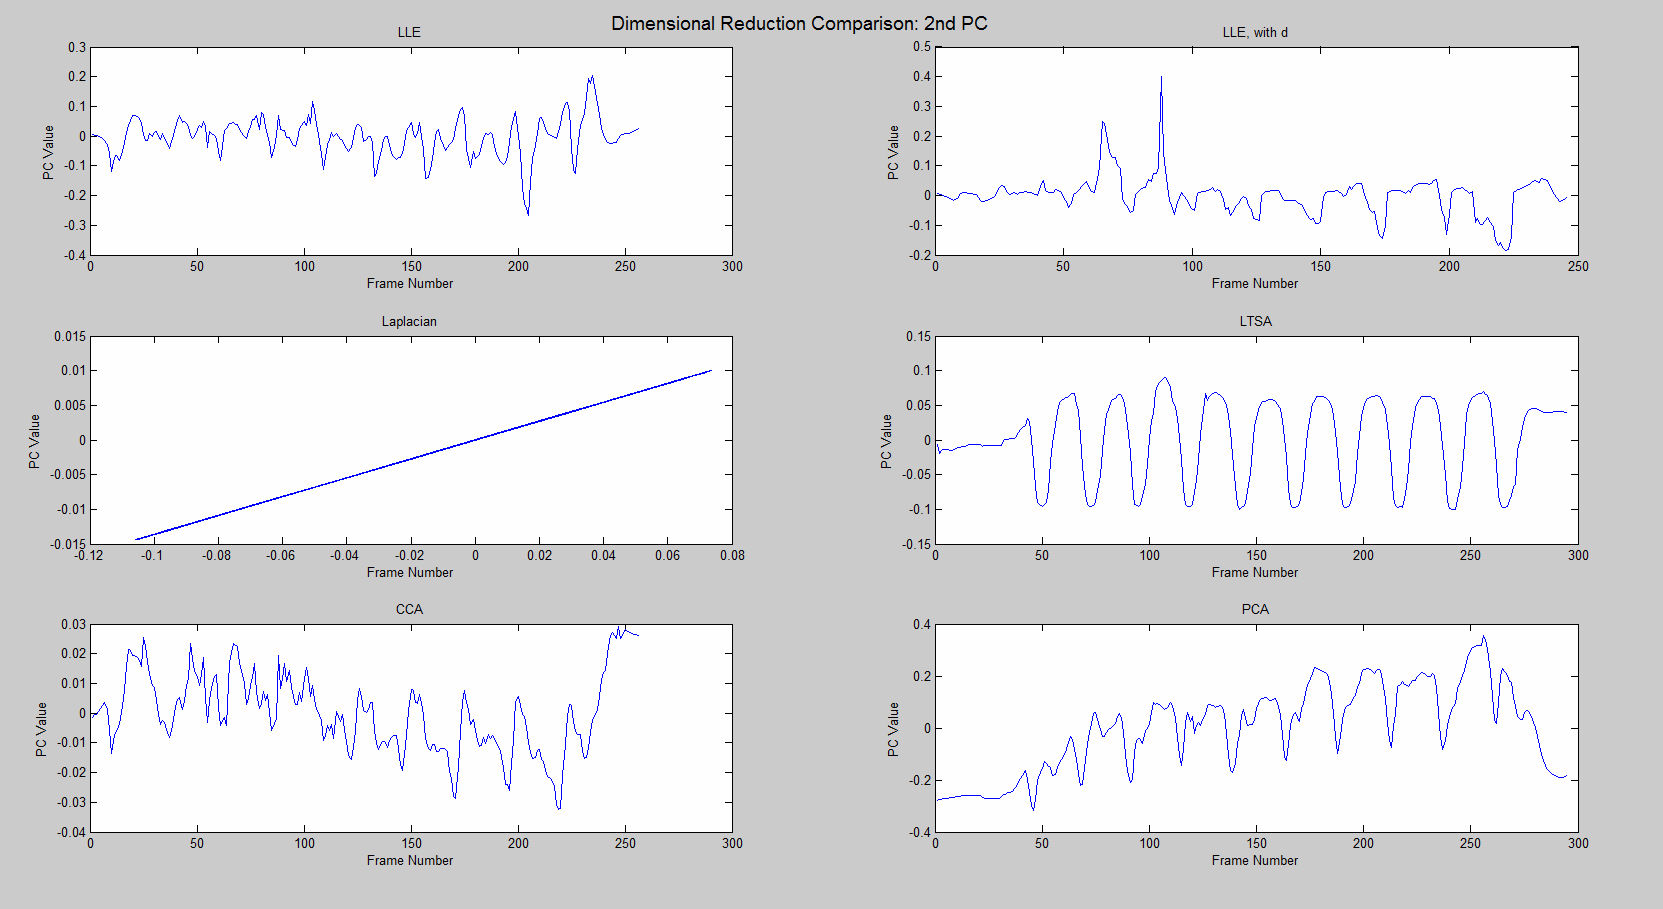
\includegraphics[height=0.25\textheight]{fig04/drcomp2.pdf}
    \mycaption[Dimensionality reduction comparison graph for PC2]{This shows the projection coefficient for the second principal component as produced by a variety of DR techniques over time}
    \label{fig:drcomp}
\end{figure}

\subsection{Pose Reconstruction}
Another benefit of using PCA is that it is possible to reconstruct the original pose using the equation $$y = U*a+Xm$$ where U is the eigenvectors, a is the projection coefficients and Xm the mean of the original data. Since we are going from low dimensionality data back to high dimensionality data it is inevitable there will be some reconstruction error. However by plotting this reconstruction along with the original it is possible to visualise how closely the lower dimensionality representation generated represent the original. This is crucial because the decomposition can be verified to make sure that important information is not lost during the reduction process.\qquad


\section{Punch Segmentation Algorithm}
After failing to find a way to automatically segment punches using existing methods It became apparent that a custom algorithm will be needed for this task, which can be broken down into several steps.

\begin{enumerate}[noitemsep]
  \item Perform PCA on raw data.
  \item Smooth the principal coefficients.
  \item Find the local maxima and minima for the punch sequence.
  \item Remove erroneous Minima\/Maxima using heuristic rules.
  \item Take a number of evenly spaced samples from between two maximum points, the length of one punch.
  \item Fetch all PCA components that correspond to the time the samples were taken.
  \item Train classifier on new data.
\end{enumerate}

Each frame representing 20 joint positions is reduced from 60 dimensions to 3 principal components per frame. Next the principal components are smoothed to remove any local minima/maxima *wrong minima/maxima*} which would prevent the automated segmentation of punches. All remaining maxima are then passed through a set of heuristic rules that checks the location of a maxima point relative to it's neighbourhood points to determine if it is legitimate. The simplest form of this is using the Pythagorean theorem to calculate the distance between a maxima and it's neighbours, if the distance is too small it is clear that one of the points is erroneous and that only one of these will be necessary for segmentation. Likewise if a neighbour is too far away it becomes obvious that one of the maxima is incorrect and needs to be removed.Thresholding is also used for each punch, with all maxima below a certain threshold removed since the cyclical signature of the punch guarantees the end of the punch will be approximately close to the end of the last punch.
\begin{figure}[h]
\hspace{-1.5cm}
\centering
\begin{minipage}{6.0cm}
    \centering
    \subtop[]{\includegraphics[height=0.25\textheight]{fig04/fig04}}
    \label{fig:kinect2}
\end{minipage}
\hspace{1.0cm}
\begin{minipage}{6.0cm}
    \centering
    \subtop[]{\includegraphics[height=0.25\textheight]{fig04/fig10}}
    \label{fig:kinect3}
\end{minipage}
\qquad
\qquad
\centering
\begin{minipage}{3.5cm}
    \centering
    \subtop[]{\includegraphics[height=0.15\textheight]{fig04/fig05}}
    \label{fig:kinect3}
\end{minipage}
\mycaption[Punch segmentation graphs]{(a) The projection coefficient of the 1st PC of a Jab sequence over time with local maxima/minima labelled. 
(b) Smoothed sequence with maxima/minima correctly identified. (c) A close up example of multiple local minima/maxima making segmentation difficult.}
\end{figure}
\clearpage

\begin{figure}[t]
 % \hspace{-1.5cm}
\begin{flushleft}
\centering
\begin{minipage}{6.0cm}
    \centering
    \subtop[]{\includegraphics[height=0.25\textheight]{fig04/rp1-crop}}
    \label{fig:a}
\end{minipage}
\hspace{2.0cm}
\begin{minipage}{6.0cm}
    \centering
    \subtop[]{\includegraphics[height=0.25\textheight]{fig04/rp2-crop}}
    \label{fig:b}
\end{minipage}
\qquad
% \centering
\begin{minipage}{6.0cm}
    \centering
    \subtop[]{\includegraphics[height=0.25\textheight]{fig04/rp3-crop}}
    \label{fig:a}
\end{minipage}
\hspace{2.0cm}
\begin{minipage}{6.0cm}
    \centering
    \subtop[]{\includegraphics[height=0.25\textheight]{fig04/rp4-crop}}
    \label{fig:b}
\end{minipage}
\qquad
\centering
\begin{minipage}{6.0cm}
    \centering
    \subtop[]{\includegraphics[height=0.25\textheight]{fig04/rp5-crop}}
    \label{fig:a}
\end{minipage}
\hspace{2.0cm}
\begin{minipage}{6.0cm}
    \centering
    \subtop[]{\includegraphics[height=0.25\textheight]{fig04/rp6-crop}}
    \label{fig:b}
\end{minipage}
\qquad
\end{flushleft}
\mycaption[Comparison of original pose and reconstructed pose]{Each graph represents a single pose with the original data in green and the reconstructed data in red obtained from back propagation.
{\bf(a)} Jab  {\bf(b)} Cross {\bf(c)} Left-Hook {\bf(d)} Right-Hook {\bf(e)} Left-Uppercut {\bf(f)} Right-Uppercut}
\end{figure}

\begin{figure}[h]
\hspace{-1.5cm}
\centering
\begin{minipage}{6.0cm}
    \centering
    \subtop[]{\includegraphics[height=0.25\textheight]{fig04/pc1}}
    \label{fig:kinect2}
\end{minipage}
\hspace{1.0cm}
\begin{minipage}{6.0cm}
    \centering
    \subtop[]{\includegraphics[height=0.25\textheight]{fig04/pc2}}
    \label{fig:kinect3}
\end{minipage}
\qquad
\centering
\begin{minipage}{6.0cm}
    \centering
    \subtop[]{\includegraphics[height=0.25\textheight]{fig04/pc3}}
    \label{fig:kinect3}
\end{minipage}
\mycaption[Graphs of the projection coefficient for the first principal component of distance \& velocity]{These figures shows the projection coefficient for the first principal component for distance data (green) and
velocity data(red).
(a) first projection coefficient (b) second projection coefficient (c) third projection coefficient}
\end{figure}

\section{Classification}

DTW
After using dynamic time warping I found that there was not enough difference between the various punch signals to give me an effective way at segmentation. Comparing jabs to other jabs yielded similarity values from $0 - 1.589$ with an average difference of $0.499$, comparing jabs to crosses yielded similarity values from $0-2.113$ with the average $0.716$. Therefore there was not enough of a consistent difference score to be able to classify they type of punch using this method.

FFT
 I investigated the possibility of running a fast Fourier transform (FFT) on the raw data as well as each segmented punch that was later obtained from using PCA and my own segmentation algorithm. The range for the coefficients was $0 - (63.030 - 0i)$ with a spread across all of the different types of punches. 
Unfortunately this meant the coefficients obtained in both cases proved to be a poor differentiator between punches due to the coefficients being so variable even within the same punch types.

PCA

Once the data has been successfully segmented into individual punches we can begin to extract features that can be used to train a classifier. Between 12 and 15 evenly spaced samples are taken for each individual punch, depending on the classifier to be used later. Each sample corresponds to a point in time which is used to extract the 3 principal coefficients for each point which results in a $36 - 45$ features for each punch.

Once all the different punch sequences are sampled for each type of punch we can use this data to train a classifier. A multi-class SVM, decision tree, Random Forest and neural network were tested. .............

Results


\section{Difficulties}
I found this project to be an excellent way to combine my interest in boxing with my Computer Science background. It was however a difficult project and I ran into a few problems.

\paragraph{Normalisation}
